\documentclass[conference]{IEEEtran}
\usepackage{amsmath,amssymb,amsthm,bm}
\usepackage{booktabs}
\usepackage{graphicx}
\usepackage{cite}
\usepackage[hidelinks]{hyperref}
\graphicspath{{images/}}
\newtheorem{proposition}{Proposition}

\title{Lost Opportunity Costs Under Ramp Stress:\\
A Comparison of Ramp-Product Dispatch and Look-Ahead Economic Dispatch}
\author{\IEEEauthorblockN{Aidan Looney, Qian Zhang, and Le Xie}
\IEEEauthorblockA{
Harvard John A. Paulson School of Engineering and Applied Sciences\\
Allston, MA, USA\\
Email: \{aidanlooney, qianzhang\}@g.harvard.edu, xie@seas.harvard.edu
}}

\begin{document}
\maketitle

\begin{abstract}
This paper studies whether ramp-product settlement compensates generators that absorb intertemporal ramp scarcity as effectively as look-ahead economic dispatch. We evaluate this question by comparing the lost opportunity cost (LOC) induced by each approach. Using rolling-horizon simulations on a 10-generator system and a modified RTS-GMLC system, we compare ramp-product settlement (RP-LMP), look-ahead settlement (LA-LMP), and temporal locational marginal pricing (TLMP). In the featured deterministic stress cases, aggregate LOC is higher under RP-LMP than under LA-LMP. The main contribution is a generator-level critical assessment for ramp-product settlement: we identify which units are left with uncompensated intertemporal opportunity cost under RP-LMP and how that burden changes under LA-LMP. RP-LMP LOC is concentrated on units with repeated ramp-binding exposure, while LA-LMP mainly relieves those same units. Multi-day tests preserve this ordering under perfect foresight in the larger system, but show that it need not hold under forecast error.
\end{abstract}

\begin{IEEEkeywords}
electricity market design, flexible ramping products, look-ahead economic dispatch, lost opportunity cost
\end{IEEEkeywords}

\section{Introduction}
As more renewable generation is integrated into electricity grids, net load (total load minus renewable generation) becomes increasingly variable. Generator ramp limits create an intertemporal coupling in real-time dispatch: a generator's current output affects its feasible output in later intervals. When these constraints bind, current-interval energy prices may fail to compensate generators for the flexibility they forgo by following dispatch, leading to incentive misalignment and lost opportunity cost (LOC).

Independent System Operators (ISOs) address system-wide ramping in two broad ways. One augments single-interval dispatch with ramping products co-optimized with energy (RP), preserving a largely myopic market structure while enforcing forward-looking feasibility. The other solves a multi-interval look-ahead economic dispatch (LAED), explicitly modeling the dispatch trajectory over a finite horizon. While both approaches incorporate intertemporal constraints into dispatch, generator settlement may still fail to price those intertemporal outcomes properly, even when a separate ramp product is cleared \cite{Zhang2026_PSCC}.

These approaches connect to three strands of literature. First, flexible ramping products and related designs have been studied as practical tools for managing renewable variability and short-term uncertainty while retaining single-interval pricing frameworks \cite{ela2016,Wang2017_review,CWang2017,wu2016,Chen2017,Chen2023}. Second, multi-interval dispatch formulations explicitly capture intertemporal feasibility by optimizing over a look-ahead horizon, but introduce more complex economic interpretations of prices due to intertemporal constraints \cite{Hua2019,Zhao2020,Scott2019,mickey2015mirtm}. Third, several pricing methods have been proposed to address intertemporal pricing, such as price-preserving pricing (PMP), constraint-preserving pricing (CMP), multi-settlement LMP (MLMP), and temporal locational marginal pricing (TLMP)\cite{hogan2020,Hua2019,Zhao2020,Guo2021}.

The key problem is therefore not only whether a ramp-product market preserves short-horizon feasibility, but whether it compensates the generators that actually absorb intertemporal scarcity as effectively as a look-ahead dispatch. We study this question using ex-post LOC, where each generator evaluates self-dispatch against the realized price trajectory \cite{Cho2023}, in a common rolling-horizon comparison of RP-LMP, LA-LMP, and TLMP.

We ask two central questions: which generators experience the highest LOC, and how does that burden change when dispatch moves from RP-LMP to LA-LMP? Unlike prior comparative studies focused mainly on operational reliability under these two dispatch methods \cite{Zhang2026_PSCC}, this paper contributes a pricing and generator-level incidence analysis. RP-LMP and LA-LMP are therefore evaluated as integrated dispatch--settlement designs; their LOC difference is not interpreted as the isolated causal effect of either look-ahead dispatch or pricing. The key innovation is to characterize how the two designs assign uncompensated ramp-scarcity costs across individual generators, rather than only comparing feasibility or total system cost. A product can procure ramp capability and still leave the opportunity cost concentrated on a small set of generators if the settlement does not price the intertemporal value of their dispatch trajectory. The contribution is threefold. First, we compare RP-LMP, LA-LMP, and TLMP in one rolling-horizon simulation framework and use ex-post LOC as a common diagnostic of uncompensated intertemporal value. Second, we decompose aggregate LOC into dispatch inefficiency and a price-support gap, clarifying why look-ahead dispatch can reduce but not eliminate LOC under uniform energy settlement. Third, we identify generator-level exposure features, especially binding frequency scaled by flexibility, that explain which units bear the RP-LMP burden and which receive LA-LMP relief. We test this incidence pattern on both the 10-generator system and a modified RTS-GMLC system.

\section{Dispatch Formulations and Pricing Rules}
\label{sec:models}
Consider a single-bus real-time dispatch problem. Let $\mathcal{G}=\{1,\dots,G\}$ denote the set of generators indexed by $g$ and let $\mathcal{W}=\{0,1,\dots,W\}$ indexed by $\tau$ denote the current interval and the advisory intervals in a rolling-window formulation. Demand at time $t+\tau$ is denoted by $d_{t+\tau}$, generator output by $p_{g,t}$ with $\tau=0$ for the ramp-product formulation (denoted just by $p_g$), and load shedding by $s_{t+\tau}\ge 0$. Each generator $g$ has linear marginal cost $c_g$, capacity bounds $\underline P_g=0,\overline P_g$, and upward and downward ramp limits $\overline{R}_g,\underline{R}_g$ per 5-minute dispatch interval. In the single-interval RP formulation, the previous realized output enters as data and is denoted by $p_{g,t-1}$. The value of lost load is denoted by $\rho$.

\subsection{Single-Interval Dispatch with Ramp Products}
The first dispatch method is a single-interval economic dispatch with co-optimized 10-minute ramp-capability products. The current dispatch decision is $p_g$, while $r^u_g$ and $r^d_g$ denote awarded upward and downward ramp-capability products. We model a simplified market-wide ramp-capability requirement, rather than a full ISO reserve-demand-curve implementation:
\begin{align}
\min_{p,r^u,r^d,s,z^u,z^d} \quad
& \sum_{g\in\mathcal{G}} c_g p_g + \rho s_t + \kappa^u z_t^u + \kappa^d z_t^d \label{eq:rp_obj}\\
\text{s.t.}\quad
& \sum_{g\in\mathcal{G}} p_g = d_t - s_t \label{eq:rp_balance}\\
& -\underline R_g \le p_g - p_{g,t-1} \le \overline R_g, \qquad \forall g \label{eq:rp_prev}\\
& 0 \le r^u_g \le K \overline R_g, \qquad \forall g \label{eq:rp_ru}\\
& 0 \le r^d_g \le K \underline R_g, \qquad \forall g \label{eq:rp_rd}\\
& p_g + r^u_g \le \overline P_g, \qquad \forall g \label{eq:rp_head}\\
& p_g - r^d_g \ge \underline P_g, \qquad \forall g \label{eq:rp_foot}\\
& \sum_{g\in\mathcal{G}} r^u_g + z_t^u \ge R_t^{u,\mathrm{req}} \label{eq:rp_sysu}\\
& \sum_{g\in\mathcal{G}} r^d_g + z_t^d \ge R_t^{d,\mathrm{req}} \label{eq:rp_sysd}\\
& s_t, z_t^u, z_t^d \ge 0, \qquad
  p_g, r^u_g, r^d_g \ge 0,\ \forall g \in \mathcal{G}. \label{eq:rp_shed}
\end{align}
Here $K=2$, representing two 5-minute intervals and therefore a 10-minute ramping product. The market-wide product requirements are constructed as
\begin{align}
R_t^{u,\mathrm{req}} = V_t^u + U_t^u, \qquad
R_t^{d,\mathrm{req}} = V_t^d + U_t^d, \label{eq:rp_req}
\end{align}
where $V_t^u,V_t^d$ are forecasted net-load-change components and $U_t^u,U_t^d$ are uncertainty adders. Following MISO \cite{MISO2026RCPUncertainty}, $U_t^u$ proxies its upward uncertainty adder, set either in MW or as $\beta\bar d$; values are not calibrated MISO requirements, and $U_t^d=0$. In the implementation used for the reported results,
\begin{align}
V_t^u = \max\{0, \widehat d_{t+K|t}-d_t\}, \\
V_t^d = \max\{0, d_t-\widehat d_{t+K|t}\} \label{eq:rp_var}
\end{align}
where $\widehat d_{t+K|t}$ is the 10-minute-ahead net-load forecast. The shortage costs $\kappa^u,\kappa^d$ are a single-segment scarcity proxy; in all reported simulations, $\kappa^u=\kappa^d=\$65/\text{MWh}$, anchored to the spinning-reserve violation cost in \cite{Chen2023}.

This RP formulation preserves the economic distinction between a single-interval capability market and multi-interval dispatch, but it is not a reproduction of an ISO implementation: it omits network and zonal requirements, multi-segment demand curves, eligibility and deployment rules, and other reserve products. Accordingly, the headline RP-LMP/LA-LMP difference compares complete dispatch-and-settlement bundles, not a pure pricing or horizon effect; matched ablations below separate these channels.


The generator settlement considered for this formulation pays current-interval energy at the balance price and awarded ramp capability at the system-wide ramp-product prices:
\begin{align}
\Pi_g^{RP}=\sum_t \left(\lambda_t^{RP} p_{g,t} + \nu_t^{u} r^u_{g,t} + \nu_t^{d} r^d_{g,t} - c_g p_{g,t}\right)\Delta t, \label{eq:rp_lmp}
\end{align}
where $\lambda_t$, $\nu_t^{u}$, and $\nu_t^{d}$ are the shadow prices on \eqref{eq:rp_balance}, \eqref{eq:rp_sysu} and \eqref{eq:rp_sysd} respectively. This price settlement models the co-optimization of the energy dispatch and ramp product market.

\subsection{Look-Ahead Economic Dispatch}
The look-ahead dispatch optimizes the full trajectory over the rolling horizon with re-optimization as the window rolls:
\begin{align}
\min_{p_{g,t+\tau},s_{t+\tau}} \quad
& \sum_{\tau\in\mathcal{W}}\left(\sum_{g\in\mathcal{G}} c_g p_{g,t+\tau} + \rho s_{t+\tau}\right) \label{eq:la_obj}\\
\text{s.t.}\quad
& \sum_{g\in\mathcal{G}} p_{g,t+\tau} = d_{t+\tau} - s_{t+\tau}, \qquad \forall \tau \label{eq:la_balance}\\
& \underline P_g \le p_{g,t+\tau} \le \overline P_g, \qquad \forall g,\tau \label{eq:la_cap}\\
& p_{g,t+\tau} - p_{g,t+\tau-1} \le \overline R_g, \qquad \forall g,\tau \label{eq:la_ru}\\
& p_{g,t+\tau-1} - p_{g,t+\tau} \le \underline R_g, \qquad \forall g,\tau \label{eq:la_rd}\\
& p_{g,t+\tau} \geq 0 \ \forall g, \tau\qquad s_{t+\tau} \ge 0, \  \forall \tau. \label{eq:la_shed}
\end{align}
The realized dispatch in the rolling simulation is the current-period component $p_{g,t}^{\star}$; the optimization is then advanced one interval and resolved with updated initial conditions.

We study two settlements for LAED.

\paragraph{LA-LMP}
The first is the current-period advisory LMP,
\begin{align}
\pi_t^{LA} = \lambda_t^{LA}, \label{eq:la_lmp}
\end{align}
where $\lambda_t^{LA}$ is the shadow price of the current-period balance equation in \eqref{eq:la_balance}.

\paragraph{TLMP}
The second is TLMP. In the single-bus setting, the generator-specific TLMP at time $t$ can be written as
\begin{align}
\pi_{g,t}^{TLMP} = \lambda_t^{LA} + \left(\overline\mu_{g,t+1}-\underline\mu_{g,t+1}\right) - \left(\overline\mu_{g,t}-\underline\mu_{g,t}\right), \label{eq:tlmp}
\end{align}
where $\overline\mu_{g,t}$ and $\underline\mu_{g,t}$ are the dual variables associated with the ramping constraints \eqref{eq:la_ru} and \eqref{eq:la_rd}. TLMP is discriminatory and internalizes generator-specific ramping shadow values such that under convexity, it yields zero LOC \cite{Guo2021}.

\section{Lost Opportunity Cost and Generator-Level Explanatory Features}
\label{sec:loc}
We evaluate each settlement rule by comparing realized generator profit under ISO dispatch to profit under self-dispatch at the same price sequence. This ex-post metric is not a behavioral bidding model; it identifies which units are left with uncompensated intertemporal value after following dispatch.

\subsection{Generator Profit Maximization Problem}
For the energy-only settlements, each generator faces a realized settlement sequence $\pi_g = \{\pi_{g,t}\}_{t=1}^T$. Under LA-LMP this sequence is uniform across units, with $\pi_{g,t}^{LA}\equiv \lambda_t^{LA}$, while under TLMP it is generator specific as in \eqref{eq:tlmp}. The generator best-response formulation is: 
\begin{align}
Q_g(\pi_g) := \max_{q_{g,t}} \quad
& \sum_{t=1}^T \left( \pi_{g,t} - c_g \right) q_{g,t}\Delta t \label{eq:gen_br_obj}\\
\text{s.t.}\quad
& \underline P_g \le q_{g,t} \le \overline P_g, \qquad \forall t \label{eq:gen_cap}\\
& -\underline R_g \le q_{g,t} - q_{g,t-1} \le \overline R_g, \qquad \forall t \label{eq:gen_ramp}
\end{align}
with initial condition $q_{g,0}$ given.

For RP-LMP, the generator also responds to the ramp-product prices. The corresponding self-scheduling problem is
\begin{align}
Q_g^{RP}:= \max_{\substack{q_{g,t},\\u_{g,t},d_{g,t}}} 
& \sum_{t=1}^T \left[(\lambda_t^{RP}-c_g) q_{g,t} + \nu_t^{u} u_{g,t} + \nu_t^{d} d_{g,t}\right]\Delta t \label{eq:gen_br_rp_obj}\\
\text{s.t.}\quad
& -\underline R_g \le q_{g,t} - q_{g,t-1} \le \overline R_g, \qquad \forall t \label{eq:gen_br_rp_ramp}\\
& 0 \le u_{g,t} \le K\overline R_g, \ 0 \le d_{g,t} \le K\underline R_g, \qquad \forall t \label{eq:gen_br_rp_prod}\\
& q_{g,t} + u_{g,t} \le \overline P_g, \ q_{g,t} - d_{g,t} \ge \underline P_g, \qquad \forall t. \label{eq:gen_br_rp_head}
\end{align}

\subsection{Realized Profit and Lost Opportunity Cost}
Let $p_{g,t}^{*}$ denote the dispatch assigned by the ISO under a given market design. For the energy-only settlements $m\in\{\mathrm{LA},\mathrm{TLMP}\}$, realized profit is
\begin{align}
\Pi_g^{\mathrm{disp},m} = \sum_{t=1}^T \left( \pi_{g,t}^{m} p_{g,t}^{*,m} - c_g p_{g,t}^{*,m} \right)\Delta t. \label{eq:profit_energy_only}
\end{align}
Under RP-LMP, realized profit includes both energy and ramp-product revenues:
\begin{align}
\Pi_g^{\mathrm{disp},RP} = \sum_{t=1}^T \left[(\lambda_t^{RP}-c_g)p_{g,t}^{*,RP} + \nu_t^{u} r_{g,t}^{u} + \nu_t^{d} r_{g,t}^{d}\right]\Delta t. \label{eq:profit_rp}
\end{align}

The ex-post lost opportunity cost (LOC) is the difference between best-response profit and realized profit $(m \in \{\text{LA}, \text{TLMP}\})$:
\begin{align}
LOC_g^{RP} := Q_g^{RP} - \Pi_g^{\mathrm{disp},RP},
LOC_g^{m} := Q_g(\pi_g^m) - \Pi_g^{\mathrm{disp},m} \label{eq:loc_def}
\end{align}

\begin{proposition}\label{prop:loc_decomp}
For any feasible dispatch $p$ that serves a fixed demand path $d$ with no load shedding under a common energy-price vector $\pi$,
\begin{align}
\sum_g LOC_g(p,\pi)
=
\underbrace{C(p)-C^\star}_{\text{dispatch inefficiency}}
+
\underbrace{\sum_g Q_g(\pi)-\pi^\top d + C^\star}_{\text{price support gap}}
\label{eq:loc_decomp}
\end{align}
where $C(p):=\sum_{g,t} c_g p_{g,t}\Delta t$, $\pi^\top d:=\sum_t\pi_t d_t\Delta t$, and $C^\star$ is the minimum feasible production cost for $d$. The identity follows from
\begin{align}
\sum_g LOC_g
&=\sum_g Q_g(\pi)-\left(\pi^\top d-C(p)\right) \nonumber\\
&=\left(C(p)-C^\star\right)
+\left(\sum_g Q_g(\pi)-\pi^\top d+C^\star\right). \nonumber
\end{align}
It applies directly to common energy-price settlements; RP product revenues are handled separately in \eqref{eq:profit_rp}.
\end{proposition}

Equation \ref{eq:loc_decomp} separates a dispatch effect from a price-support effect. LAED can reduce the first term by improving the implemented trajectory, but uniform current-interval prices cannot eliminate the second term when ramp constraints bind. TLMP removes this residual gap by embedding the generator-specific marginal value of ramping constraints into the settlement price.

\subsection{Generator-Level Explanatory Features}
To characterize cross-generator heterogeneity in LOC, we screen features constructed from the realized trajectories:
\begin{itemize}
    \item \textbf{Flexibility ratio:} $\mathrm{flex}_g=R_g/\overline P_g$.
    \item \textbf{Bind frequency:} the fraction of realized ramp movements that are nearly binding.
    \item \textbf{Flex-adjusted bind exposure:} $\mathrm{bind}_g/\mathrm{flex}_g$.
\end{itemize}
The multivariate analysis also controls for capacity, marginal cost, and realized utilization.

\section{Simulation Design}
\label{sec:setup}
\subsection{Rolling-Horizon Structure}
All dispatch problems use a deterministic, single-bus rolling-horizon simulation with 5-minute settlement intervals. At time $t$, the chosen dispatch model is solved over a look-ahead horizon, only the current dispatch decision is implemented, and the horizon is rolled forward. This setup uses a single-bus setting to isolate intertemporal ramping effects. Generator costs are linear, and the value of lost load is fixed at \mbox{\$3{,}500/MWh} \cite{Chen2023}.

\subsection{Test System}
The reported results use two test systems. The first is a heterogeneous 10-generator system with varying costs, capacities, and ramp rates; Table~\ref{tab:gen_loc_example} reports its parameters together with the severe-case generator LOC results. The second is a controllable single-bus reduction of the RTS-GMLC system \cite{Barrows2020RTS}, containing 93 generators.

\begin{table}[!t]
\caption{Generator parameters and severe-case LOC. Cost is in dollars/MWh; capacity and 5-min ramp limit are in MW; LOC is in dollars. $\Delta LOC:=LOC_g^{LA}-LOC_g^{RP}$.}
\label{tab:gen_loc_example}
\centering
\small
\setlength{\tabcolsep}{1.6pt}
\begin{tabular}{crrrrrrr}
\toprule
Gen. & Cost & Cap. & Ramp & RP LOC & LA LOC & TLMP & $\Delta LOC$ \\
\midrule
1  & 185.0 & 22  & 7.5  & 0.0    & 0.0             & 0 & 0.0 \\
2  & 30.0  & 170 & 17.5 & 663.2  & \textbf{77.9}   & 0 & -585.4 \\
3  & 55.0  & 85  & 7.5  & \textbf{52.5} & 101.6    & 0 & 49.1 \\
4  & 15.0  & 230 & 7.5  & 42.8   & \textbf{0.0}    & 0 & -42.8 \\
5  & 20.0  & 613 & 37.5 & 0.0    & 0.0             & 0 & 0.0 \\
6  & 19.5  & 686 & 10.0 & 3487.3 & \textbf{1984.1} & 0 & -1503.3 \\
7  & 48.0  & 45  & 10.0 & 47.0   & \textbf{8.9}    & 0 & -38.1 \\
8  & 60.0  & 50  & 5.0  & \textbf{0.0} & 5.7      & 0 & 5.7 \\
9  & 57.0  & 260 & 5.0  & \textbf{10.4} & 27.1    & 0 & 16.7 \\
10 & 50.0  & 400 & 12.5 & 4129.8 & \textbf{278.0}  & 0 & -3851.8 \\
\midrule
\multicolumn{4}{r}{Total LOC} & 8433.1 & \textbf{2483.1} & 0 & -5950.0 \\
\bottomrule
\end{tabular}
\end{table}

We study three uniform ramp-scaling regimes for the 10-generator system: 0.8, 0.2, and 0.1 of the base ramp capability. The demand trajectory is held fixed while ramp capability is scaled, isolating ramp scarcity. The paper focuses on the 0.1 ramp factor because it produces clear intertemporal scarcity and generator-level LOC heterogeneity while remaining feasible.

\subsection{Implementation Notes}
The reported figures and tables use the deterministic 10-generator 0.1 ramp factor scenario with a 1-hour look-ahead horizon. The load trajectory is the August 2032 projection from MISO, scaled to a 1{,}100 MW reference capacity over the course of a whole day. The publication models are linear programs solved with SciPy/HiGHS.

The featured 10-generator RP case uses $U_t^u=40$ MW as a fixed proxy for MISO's upward uncertainty adder, $U_t^d=0$, and $\kappa^u=\kappa^d=\$65/\text{MWh}$ following \cite{Chen2023}. The RTS-GMLC benchmark aggregates an 8-hour high-ramp window from 2020-06-11, scales peak load to 95\% of controllable capacity, and uses ramp factor 0.6. Its base case sets $U_t^u=U_t^d=0$ to isolate $V_t^u,V_t^d$; the ramp-product requirements still equal those forecasted net-load changes.

Separate robustness checks use 28 full-day RTS-GMLC net-load profiles (seven January, April, July, and October days), scaled to 1{,}100 MW mean for the 10-generator system. This grid varies ramp multipliers $\{0.1,0.2,0.4,0.8\}$, upward-adder fractions $\beta\in\{0,0.08,0.16,0.24\}$ with $U_t^u=\beta\bar d$, LAED horizons $\{1,3,7,13\}$, and error scales $\{0,1,3,5\}\%$. Forecasts use stationary Gaussian AR(1) delivery-time paths ($\rho=0.9$), shared by both designs and retained as windows roll; scale grows with the square root of lead time, capped after four intervals, with three seeds per nonzero level. On RTS-93, 12 days test ramp factors $\{0.2,0.4,0.8\}$; separate horizon and AR(1) checks use 0.3 and 0.6, respectively.

\section{Results}
\label{sec:results}
\subsection{Cross-Regime Summary}
On the featured day, tightening the ramp factor from 0.8 to 0.2 and 0.1 increases the share of generator ramp transitions at their limits from 0 to 0.40\% and 3.59\%. Across the same three ramp factors, RP-LMP LOC is 0, 187.4, and 8{,}433.1, while LA-LMP LOC is 0, 7.5, and 2{,}483.1. In the most severe case, there is no load shedding, 99 ramp transitions reach their limits, and the RCUP price is positive in 10.5\% of intervals, reaching \mbox{\$40/MWh}. The largest difference between TLMP and the energy price is \mbox{\$44/MWh}.

In the severe case, LA-LMP cuts total LOC by 70.6\%, from 8{,}433.1 to 2{,}483.1. It therefore reduces LOC substantially, but does not eliminate it. The remaining LOC arises because a single uniform energy price does not fully compensate every generator for the opportunity cost created by ramp constraints.

When ramp constraints do not bind at ramp factor 0.8, both RP-LMP and LA-LMP produce zero LOC. LOC appears as ramp capability tightens, showing that the burden is driven by binding ramp constraints rather than by the presence of a ramp product alone.

Because RP-LMP and LA-LMP differ in both dispatch and settlement, matched comparisons examine each channel on an independent full-day profile. Holding RP dispatch fixed, adding ramp-capability revenue reduces LOC from 10{,}521 to 5{,}417. Holding uniform LA-LMP settlement fixed, extending LAED from one to 13 intervals reduces LOC from 5{,}572 to 280. These checks show that both channels affect LOC, although they do not provide a complete decomposition of the headline difference.

\subsection{Which Generators Bear the LOC Burden?}
Unless noted otherwise, results below refer to the 10-generator low ramp scenario. Table~\ref{tab:gen_loc_example} shows that TLMP eliminates LOC, whereas RP-LMP and LA-LMP leave positive LOC for some generators and neither produces lower LOC for every generator.

Although total LOC is lower under LA-LMP, not every generator benefits. LA-LMP lowers LOC for five generators, RP-LMP lowers it for three, and two are tied. Generator 10 is the clearest example: under RP-LMP its realized profit is \mbox{-\$1{,}961.1}, even though it could have earned a positive profit by choosing its own best feasible dispatch at the same prices.

Generators 10, 6, and 2 have the largest RP-LMP LOC, and generators 10 and 6 account for 90.3\% of the total. LA-LMP lowers LOC for generators 10, 6, and 2 by 3{,}851.8, 1{,}503.3, and 585.4. For the three generators with higher LOC under LA-LMP, the increases are only 49.1, 5.7, and 16.7.

LA-LMP mainly helps the generators whose ramps bind most often under RP-LMP, while causing only small increases for a few other units. Even when the RCUP price is positive, these frequently constrained generators still carry most of the RP-LMP LOC.

The larger RTS-GMLC system shows similar concentration. Positive LOC occurs for 55 of 93 generators under RP-LMP and 26 under LA-LMP. Only 11 generators have higher LOC under LA-LMP, by an average of \mbox{\$3.30}. In both designs, the largest burdens fall on a small group of gas combined-cycle units.

\subsection{What Drives LOC Across Generators?}
Figure~\ref{fig:dispatch_compare} shows the operating mechanism: LAED moves frequently constrained generators earlier, reducing repeated ramp binding.

\begin{figure}[!b]
    \centering
    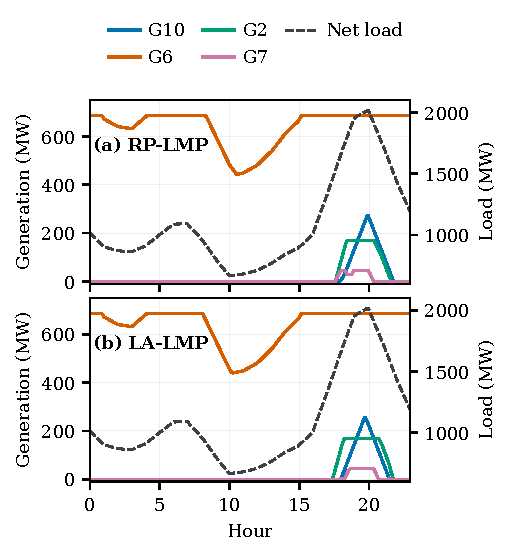
\includegraphics[width=\columnwidth,trim=0 8 0 8,clip]{images/10gen_dispatch_window_rp_vs_la.pdf}
    \caption{Full-day dispatches for four generators in the 10-generator ramp-constrained case under RP-LMP (top) and LA-LMP (bottom). The dashed line is net load. Generators 10, 6, and 2 have the largest RP-LMP LOC; generator 7 shows a smaller offsetting dispatch change under LAED.}
    \label{fig:dispatch_compare}
\end{figure}

These dispatch patterns align with generator characteristics. Generators 10, 6, and 2 have flexibility ratios of 0.031, 0.015, and 0.103, and their ramps bind in 14.3\%, 7.8\%, and 3.4\% of intervals. Generator 10 reaches its upward ramp limit in 6.9\% of intervals in which producing more would be profitable; its average price-cost margin in those intervals is \mbox{\$1.82/MWh}. Generator 6 instead has very low flexibility.

In the 10-generator severe case, flexibility ratio alone explains little of the variation in LOC ($R^2=0.158$ for RP-LMP and 0.113 for LA-LMP). For RP-LMP, ramp-bind frequency gives $R^2=0.823$, which rises to 0.849 when bind frequency is divided by flexibility. For LA-LMP, the corresponding values are 0.256 and 0.697. How often a generator's ramp binds is therefore a stronger indicator of LOC than low flexibility alone, although low flexibility makes these events more costly. These generators also receive the largest LA-LMP relief.

Figure~\ref{fig:rts_bivariate} confirms this pattern for one RTS-GMLC day. Ramp-bind frequency alone gives $R^2=0.576$ for RP-LMP LOC and 0.556 for $LOC^{LA}-LOC^{RP}$; dividing it by flexibility raises these values to 0.725 and 0.688. We then estimate two generator-day regressions across both systems using cases without load shedding or spillage (1{,}256 observations from 103 generators). The outcomes, reported in the same order below, are $\log(1+\mathrm{RP\ LOC/MW})$ and the signed log of LA-LMP relief, $(\mathrm{RP}-\mathrm{LA})$ LOC per MW. The signed log preserves the direction of the difference while limiting the influence of extreme values. Each regression includes standardized bind frequency, log flexibility, log capacity, marginal cost, utilization, and a test-system indicator; p-values use generator-clustered standard errors to account for repeated observations. Bind frequency is positive in both regressions: 0.864 ($p<0.001$) and 0.819 ($p<0.001$). Log flexibility is negative: $-0.223$ ($p=0.017$) and $-0.219$ ($p=0.019$), as is log capacity: $-0.200$ ($p=0.037$) and $-0.204$ ($p=0.034$). Marginal cost ($p=0.076$ and 0.070) and utilization ($p=0.140$ and 0.157) are not significant at the 5\% level. The regressions have $R^2=0.812$ and 0.802.

\begin{figure*}[!t]
    \centering
    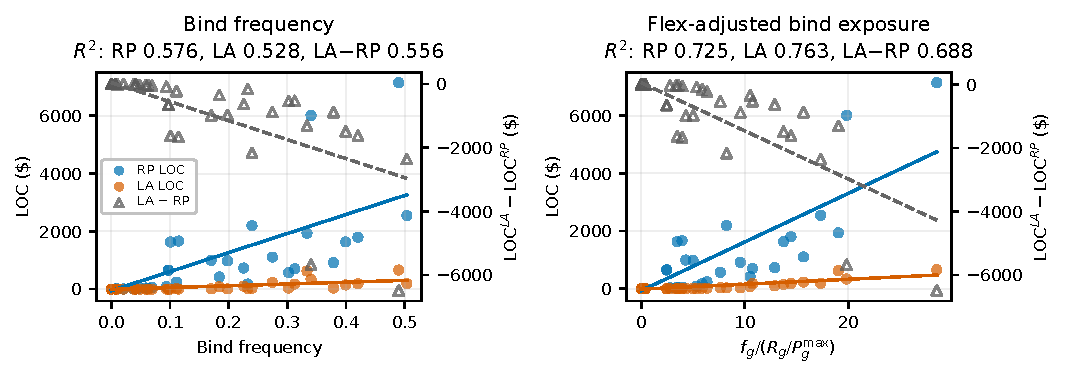
\includegraphics[width=\textwidth]{images/rts_dispatchable_laed_vs_rp_loc_bivar_ylinear.pdf}
    \caption{Generator-level LOC under RP-LMP and LA-LMP in the 93-generator controllable RTS-GMLC system, with $LOC^{LA}-LOC^{RP}$ on the right axis. The left panel uses ramp-bind frequency; the right divides bind frequency by flexibility ratio. As in the 10-generator case, RP-LMP LOC and the reduction under LA-LMP are largest for generators whose ramps bind often.}
    \label{fig:rts_bivariate}
\end{figure*}

\subsection{Validation and Forecast Sensitivity}
The larger RTS-GMLC system validates the aggregate result. At ramp multiplier 0.6, $U_t^u=0$, so the ramp requirement contains only forecasted net-load change, and both RP-LMP and LA-LMP serve all load. The RCUP price reaches \mbox{\$9.06/MWh}. Total LOC is $53{,}456.8$ under RP-LMP, $1{,}463.0$ under LA-LMP, and zero under TLMP, so the RP-LMP result is not caused by load shedding.

Table~\ref{tab:robustness_summary} summarizes the multi-day validation and forecast-sensitivity checks, omitting 10-generator ramp 0.1 because only 2/28 days avoid penalty balancing.

\begin{table}[!b]
\caption{LOC across days and settings. ``No shed/spill'' gives qualifying/total cases; $LOC^{LA}<LOC^{RP}$ gives the share satisfying that strict inequality. $\Delta=LOC^{RP}-LOC^{LA}$ is in dollars; IQR is $[Q_1,Q_3]$. $\beta$ sets the upward-adder proxy $U_t^u=\beta\bar d$.}
\label{tab:robustness_summary}
\centering
\scriptsize
\setlength{\tabcolsep}{1.8pt}
\renewcommand{\arraystretch}{0.90}
\begin{tabular}{lrrrr}
\toprule
Case & No shed/spill & $LOC^{LA}<LOC^{RP}$ & Med. $\Delta$ & IQR $\Delta$ \\
\midrule
\multicolumn{5}{l}{10-generator, perfect foresight, adder $\beta=0.16$} \\
Ramp 0.2 & 6/28 & 66.7\% & 149 & [25, 413] \\
Ramp 0.4 & 14/28 & 71.4\% & 23 & [1, 79] \\
Ramp 0.8 & 20/28 & 15.0\% & 0 & [0, 0] \\
\midrule
\multicolumn{5}{l}{10-generator, AR(1), ramp 0.2, adder $\beta=0.08$} \\
0\% error & 6/28 & 66.7\% & 149 & [25, 413] \\
1\% error & 18/84 & 50.0\% & 50 & [$-33$, 563] \\
3\% error & 19/84 & 10.5\% & $-1{,}162$ & [$-2{,}829$, $-426$] \\
5\% error & 19/84 & 0.0\% & $-10{,}603$ & [$-18{,}185$, $-8{,}855$] \\
\midrule
\multicolumn{5}{l}{RTS-93, perfect foresight, adder $\beta=0.16$} \\
Ramp 0.2 & 12/12 & 100.0\% & 62{,}199 & [52{,}313, 78{,}329] \\
Ramp 0.4 & 12/12 & 100.0\% & 31{,}981 & [18{,}144, 46{,}441] \\
Ramp 0.8 & 12/12 & 100.0\% & 8{,}330 & [3{,}754, 13{,}715] \\
\midrule
\multicolumn{5}{l}{RTS-93, AR(1), ramp 0.6, adder $\beta=0.16$} \\
0\% error & 12/12 & 100.0\% & 15{,}448 & [5{,}500, 23{,}073] \\
1\% error & 36/36 & 88.9\% & 12{,}164 & [1{,}465, 19{,}122] \\
3\% error & 36/36 & 30.6\% & $-10{,}797$ & [$-20{,}659$, 1{,}280] \\
5\% error & 36/36 & 5.6\% & $-48{,}164$ & [$-73{,}345$, $-24{,}478$] \\
\bottomrule
\end{tabular}
\renewcommand{\arraystretch}{1}
\end{table}

To isolate uncertainty in the ramp requirement from forecast error, $\beta$ scales the upward adder $U_t^u=\beta\bar d$. Across the reported ramp factors, qualifying perfect-foresight cases at every tested $\beta$ satisfy \mbox{$LOC^{LA}\le LOC^{RP}$}; the remainder are ties. For RTS-93, median LOC relief declines from 62{,}199 at ramp factor 0.2 to 31{,}981 at 0.4 and 8{,}330 at 0.8, with LA-LMP lower on all 12 days. Across ten RTS-93 days feasible at all horizons, median LA-LMP LOC falls from 50{,}634 with one interval to 23{,}876, 11{,}812, and 5{,}405 with 3, 7, and 13 intervals; RP-LMP stays at 50{,}634 because it has no look-ahead window.

In both AR(1) panels, median $LOC^{RP}-LOC^{LA}$ changes from positive to negative between 1\% and 3\% forecast error. Thus, LA-LMP has lower median LOC at the smaller error level but higher median LOC at the larger level. This compares the complete designs: LAED forecasts 13 intervals, whereas RP uses only the 10-minute forecast in its requirement. It tests forecast sensitivity, not pricing alone.

\section{Conclusion}
\label{sec:conclusion}
This paper compared RP-LMP, LA-LMP, and TLMP in a common rolling-horizon framework under ramp stress. In the featured deterministic cases, RP-LMP leaves larger aggregate ex-post LOC than LA-LMP, concentrated on generators with repeated ramp-binding exposure. LA-LMP relieves those same units but, under a uniform current-interval price, does not eliminate residual LOC; TLMP eliminates it. Multi-day perfect-foresight checks preserve the aggregate ordering in the larger system, while forecast-error tests show that it is not universal. Because the RP representation is stylized and omits network, commitment, and detailed ISO demand-curve rules, these results do not establish generic superiority of one market implementation. They instead show why ramp-product designs should be evaluated both for procured capability and for compensation of generators that repeatedly absorb intertemporal scarcity.

\section{Acknowledgment}
\emph{Disclaimer}: The views expressed in this paper are the opinion of the authors and do not reflect the views of PJM Interconnection, L.L.C. or its Board of Managers of which Le Xie is a member.

\bibliographystyle{IEEEtran}
\bibliography{references}

\end{document}
